\documentclass[a4paper, parskip=half, twopage]{scrartcl}
\usepackage[english]{babel}
\usepackage[utf8]{inputenc}
\usepackage[T1]{fontenc}

\usepackage[expansion=false, tracking=false, protrusion=true]{microtype}

\usepackage{amsmath}
\usepackage{amsfonts}
\usepackage{amssymb}

\usepackage{xfrac}

\usepackage{mhchem}

\usepackage{siunitx}

\usepackage{tikz}

%\usepackage{xfrac}

\addtokomafont{disposition}{\rmfamily}

\newcommand{\p}[1]{\frac {\partial}{\partial #1}}
\newcommand{\pd}[2]{\frac {\partial #1}{\partial #2}}
\newcommand{\pdd}[2]{\frac {\partial^2 #1}{\partial #2 ^2}}
\newcommand{\pmd}[3]{\frac {\partial^2 #1}{\partial #2 \partial #3}}

\begin{document}

\Huge \textbf{\textsc{Hand-in exercises}} \\*
\Large \textbf{Nuclear Physics}

\normalsize Per Engsström \hfill \oldstylenums{920127}-\oldstylenums{3258} \hfill \textsc{Bachelor Programme in Physics, third year} \\
\rule{\textwidth}{1pt}

\bigskip

\section*{Problem 1}
We know from the lectures and lessons that the number of nucleii as a function of time can be described by the equation
\begin{equation}
N(t) = N_0 e^{-\lambda t}
\label{decomp}
\end{equation}
where $N_0$ is the number of nucleii at $t=0$ and $\lambda$ is the decay constant. The decay constant is related to the half-life by $\lambda t_{\sfrac 1 2} = \ln 2$.

We assume that at the time of disaster, $m_0$ kilograms of \ce{^{236}U} had undergone fission in the reactor. Afterwards, no more fission takes place and no more \ce{^{131}I} or \ce{^{133}I} is produced. Thus, the initial mass of \ce{^{131}I} and \ce{^{133}I} are
\[
m_A = m(\ce{^{131}I}) = 0.02892m_0 \quad m_B = m(\ce{^{133}I}) = 0.06686m_0
\]

We can relate this to the number of nucleii by the \emph{molar mass} $\mu$. From the definition, we find $\mu$ from the number of nucleons.
\[
\mu_A = \mu(\ce{^{131}I}) = \SI{0.131}{\kg\per\mole} \quad \mu_B = \mu(\ce{^{133}I}) = \SI{0.133}{\kg\per\mole}
\]
The mass and molar mass is related to the number of moles $n$ by $n \mu = m$. In turn, the number of nucleii $N$ is simply $N = n L$ where $L$ is \emph{Avogadro's number} (approximately \SI{6.022e23}{\per\mole}).

From the \emph{Chart of Nuclides}\footnote{\texttt{http://www.nndc.gov/chart}} we see that their respective half-lives is
\[
t_{\sfrac 1 2, A} = \SI{8.03}{d} \quad t_{\sfrac 1 2, B} = \SI{20.8}{h}
\]
both isotopes decay by $\beta$-radiation. Thus any daughter nucleii would have the same number of nucleons as the parent. Additionally, the isotopes differ by 2 nuclides, meaning $\alpha$-decay wouldn't join them. This means that their respective decay chains are independent. Thus, the amount of either isotope is decreasing exponentially according to equation \ref{decomp}.

We can now write these equations
\begin{align}
N_A(t) &= N_{0,A} e^{-\lambda_A t} = \frac{m_A L}{\mu_A} e^{-\lambda_A t} \label{na} \\
N_B(t) &= N_{0,B} e^{-\lambda_B t} = \frac{m_B L}{\mu_B} e^{-\lambda_A t} \label{nb}
\end{align}

The activity $\mathcal{A} = \lambda N$ can easily be derived from equations \ref{na} and \ref{nb}. The ratio\footnote{The activity for both isotopes is considered in the same volume, so it doesn't matter.}
\[
\mathcal{K} = \frac{\mathcal{A}_A}{\mathcal{A}_B} = \frac{\SI{0.12}{\becquerel\per\cubic\metre}}{\SI{0.39}{\becquerel\per\cubic\metre}} \approx 0.31
\]
is preserved any distance from Chernobyl. To ensure ourselves this, we assume that a fraction $f$ of the fallout reaches Gothenburg, i.e. it experiences a fraction $f\mathcal{A}$ of the total activity. Now, since the composition is somewhat uniform, we can safely assume that the same fraction $f$ applies to both isotopes. Hence $f\mathcal{A}_A$ and $f\mathcal{A}_B$ are the activities of the isotopes in Gothenburg. And their ratio is simply $\mathcal{K}$, as expected.

This means that if we find $t$ for which $\mathcal{K} \approx 0.308$ we have found out how much time has elapsed since the event! Setting up the equations we get
\[
\mathcal{K} = \frac{\lambda_A N_A}{\lambda_B N_B} = \frac{\lambda_A m_A \mu_B}{\lambda_B m_B \mu_A} e^{(\lambda_B - \lambda_A) t}
\]
Note that the common factor $L$ disappears. If we solve for $t$ (and noting that the ratio of $m_A$ and $m_B$ doesn't depend on $m_0$) we get
\[
t = \frac{\ln \left[ \mathcal{K} \frac{\lambda_B m_B \mu_A}{\lambda_A m_A \mu_B} \right]}{\lambda_B - \lambda_A} \approx \SI{2.3e5}{s}
\]

This corresponds to about 2 days, 15 hours and 14 minutes. This would mean that the disaster occurred at 01:46, 26/4-1986 Swedish time. If we look up the actual time and date\footnote{\texttt{http://en.wikipedia.org/wiki/Chernobyl\_disaster}}, we find that it occurred at 00:23, 26/4-1986 Swedish time. Less than 1.5 hours from the calculated date.

\subsection*{Part B}

The plot in figure 

\section*{Problem 2}
\subsection*{Part A}
The charge distribution of a homogeneously charged sphere can be written as
\[
\rho(r) = \begin{cases}
\rho & r \leq R \\
0 & r > R \\
\end{cases}
\]
If we integrate this in all of space, we expect it to be 1. So we have
\[
A \int\limits_{\mathbb{R}^3} \rho(r) d\tau = 1
\]
for some normalization constant A. The charge distribution is zero for $r$ larger then $R$ so we need only integrate up to $R$. If we evaluate it in spherical coordinates we get
\[
A \int\limits_{\mathbb{R}^3} \rho(r) r^2 \sin \theta \, dr d\theta d\varphi = 4\pi A \rho \int\limits_{0}^{R} r^2 \, dr = \frac{4 \pi}{3} A \rho R^3 = 1, \quad A = \frac{3}{4 \pi \rho R^3} 
\]

The mean square radius $\langle r^2 \rangle$ is calculated by multiplying the integrand by $r^2$ and evaluating
\[
\langle r^2 \rangle = \frac{3}{4 \pi \rho R^3} \int\limits_{\mathbb{R}^3} r^2 \rho(r) d\tau = \frac{3}{4 \pi \rho R^3} \int\limits_{\mathbb{R}^3} \rho(r) r^4 \sin \theta \, dr d\theta d\varphi = \frac{3}{R^3} \int\limits_{0}^{R} r^4 \, dr = \frac{3}{5} R^2
\]

We define the mean radius as $\sqrt{\langle r^2 \rangle}$.

\subsection*{Part B}

The differential cross section is given by
\[
\left( \frac{d \sigma}{d \Omega} \right)_\text{exp} = \left( \frac{d \sigma}{d \Omega} \right)_\text{Rutherford} | F(q^2)|^2 \left( 1 - \beta^2 \sin^2\left( \frac{\theta}{2} \right) \right)
\]
where Rutherford's cross section in turn is given by
\[
\left( \frac{d \sigma}{d \Omega} \right)_\text{Rutherford} = \left( \frac{Z_1 Z_2 e^2}{8 \varepsilon_0 \pi E} \right)^2 \frac{1}{\sin^4 \left( \frac{\theta}{2} \right)}.
\]
From exercise 1.3 we obtain the following form factor:
\[
|F(q^2)|^2 = \left( 1-\frac{q^2}{6\hbar^2}\langle r^2 \rangle \right)^2 .
\]
By combining the equations above we get
\[
\left( \frac{d \sigma}{d \Omega} \right)_\text{exp} = \left( \frac{Z_1 Z_2 e^2}{8 \varepsilon_0 \pi E} \right)^2 \frac{1}{\sin^4 \left( \frac{\theta}{2} \right)} \left( 1-\frac{q^2}{6\hbar^2}\langle r^2 \rangle \right)^2 \left( 1 - \beta^2 \sin^2\left( \frac{\theta}{2} \right) \right)
\]
and solving for the mean square radius gives us
\[
\langle r^2 \rangle = \frac{6\hbar^2}{q^2} \left( 1 - \left( \frac{8\varepsilon_0\pi E}{Z_1 Z_2 e^2} \right) \sin^2 \left(\frac{\theta}{2} \right) \sqrt{ \frac{\left( \frac{d \sigma}{d \Omega} \right)_\text{exp}}{\left( 1 - \beta^2 \sin^2\left( \frac{\theta}{2} \right) \right)} } \right)
\]

By assuming $m_e c^2 << E$, we can assume $\beta^2 \approx 1$. Furthermore, the scattering angle is related to the transferred momentum $q = 2k\sin\left( \theta /2 \right)$ where $k = p/\hbar$ is the wave number and $p = E/c$ is the momentum. We have
\[
\sin\left( \frac{\theta}{2} \right) = \left( \frac{qc\hbar}{2E} \right)^2 .
\]
We get the value $q \approx \SI{0.5}{\per\femto\metre}$  (transferred momentum divided by $\hbar$) from figure 4.6 in the book. Similarly, we get $\left( \frac{d \sigma}{d \Omega} \right)_\text{exp} \approx \SI{10}{mb\per sr}$ For $E \approx \SI{450}{\MeV}$. For $Z_1 = 1$ and $Z_2 = 28$ we get $\langle r^2\rangle \approx \SI{1.039e-29}{\meter\square}$ and
\[
\langle r^2 \rangle^{1/2} \approx \SI{3.22}{fm}
\]
\section*{Problem 3}

We know that the count rate $R$ for the detector is related to the differential cross section by
\[
R = \pd{\sigma}{\Omega} N \Phi {\Delta\Omega}, \quad \Delta\Omega = \frac{A}{r^2}
\]
The number of \ce{^{63}Cu} atoms $N$ in the beam's way is related to the flux $\Phi$ by
\[
N = \frac{S t \rho N_A}{\mu}, \quad \Phi = \frac{I}{S}, \quad N \Phi = \frac{t \rho N_A I}{\mu}
\]
This means that the differential cross section is
\[
\pd{\sigma}{\Omega} = \frac{R \mu r^2}{t \rho N_A I A}
\]
Now we just input the numerical values. The intensity $I$ is the current divided by the elementary charge. This gives
\[
\pd{\sigma}{\Omega} (30^\circ) \approx \SI{1.1}{\milli\barn\per\steradian}
%\frac{(\SI{2400}{\sec^{-1}})
%(\SI{0.063}{\kg\per\mole})
%(\SI{0.5}{m})^2
%(\SI{1.602e-19}{\ampere\sec})}
%{(\SI{1}{\mm})
%(\SI{6.022e23}{\per\mole})
%(\SI{1}{\cm\square}
%(\SI{1e-8}{\ampere})}
\]
\section*{Problem 4}

\subsection*{Part A}

We look at the number of nucleons in each isotope. Niobium-95 consists of 41 protons and 54 neutrons. It has an unpaired proton. If we start filling out the shells we see that the unpaired proton is in $1g_{9/2}$. The parity is then positive ($(-1)^\ell = 1$ for $\ell = 4$).

Similarly for Molybden-95 we find the unpaired nucleon is in $2d_{5/2}$ with positive parity. The excitation of \ce{^{95}Mo} moves the unpaired nucleon to the $1g_{7/2}$ state of positive parity. A decay scheme can be seen below.

\begin{center}
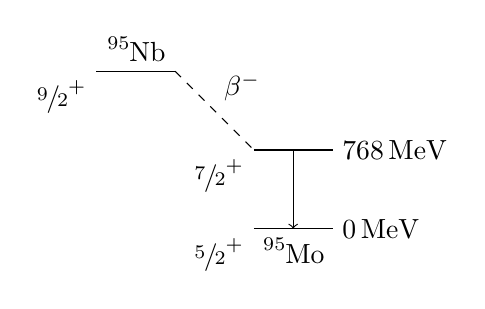
\begin{tikzpicture}
\path[draw] (0,0) node[below left] {$\sfrac{9}{2}^+$} -- node[above] {\ce{^{95}Nb}} (1,0);
\draw (2,-1) node[below left] {$\sfrac{7}{2}^+$} -- (3,-1) node[right] {\SI{768}{\MeV}};
\draw[dashed] (1,0) -- node[above right] {$\beta^-$} (2,-1);
\draw (2,-2) node[below left] {$\sfrac 5 2 ^+$} -- node[below] {\ce{^{95}Mo}} +(1,0) node[right] {\SI{0}{\MeV}};
\draw[->] (2.5,-1) -- (2.5,-2);
\end{tikzpicture}
\end{center}

\subsection*{Part B}

We look at the reaction equation:
\[
\ce{^{95}Nb -> ^{95}Mo^* + e^- + \bar{\nu} + Q}
\]
If we assume that the neutrino has zero mass and look at the energies on both sides we can solve for $Q$.
\[
(41m_p + 54m_n)c^2 - B(\ce{^{95}Nb}) = (42m_p + 53m_n)c^2 - B(\ce{^{95}Mo}) + m_e c^2 + Q
\]
\[
Q = B(\ce{^{95}Mo}) - B(\ce{^{95}Nb}) + (m_n - m_p - m_e)c^2 \approx \SI{922}{\keV}
\]
Values for binding energies taken from P.H. T-6.1.

If we assume that the only possible decay channel is to the exited \ce{^{95}Mo^*} state, then part of $Q$ must be spent exiting the nucleus. If we also assume no energy is given to the neutrino we can calculate the maximum possible $\beta$-electron energy:
\[
E_{\text{max}} = Q - E_{\text{exc}} \approx \SI{154}{\keV}
\]

The internal conversion electron is produced by expelling a electron from orbit using the excitation energy. This is most probable for the K-shell. A part of the energy must be used to overcome the electron binding energy, so the maximum is:
\[
E_{\text{\textsc{IC}}} = E_{\text{exc}} - B \approx \SI{748}{\keV}
\]

\subsection*{Part C}

The difference $\Delta J$ between the parent and exited daughter is $\Delta J = 1$. This would give $L$-values of 0 and 1. Since there is no parity change we conclude that it's and allowed Gamow-Teller $\beta$-decay.

For the $\gamma$-radiation we look at the interval $|\sfrac 7 2 - \sfrac 5 2 | \leq L \leq | \sfrac 7 2 + \sfrac 5 2 |$ or $1 \leq L \leq 6$. The lowest $L$ is the most probable, and since there is no change in parity, we see that it's most likely a M1 transition.

\section*{Problem 5}

\subsection*{Part A}
We know that for any inertial frame, $E^2 - p^2 c^2 = E'^2 - p'^2 c^2$. The momentum in the \textsc{com} frame is zero, and the momentum in the lab frame is all on the incident proton.
\[
E_{\mathrm{CM}}^2 = (m_\mathrm{i} + m_p)^2 c^4 - p_\mathrm{i}^2 c^2
\]
for relativistic mass $m_\mathrm{i}$.

The least energy needed is $E_\mathrm{CM} = 4 m_p c^2$. Inserting this in the above equation gives
\[
16 m_p c^2 = m_\mathrm{i}^2 c^4 + m_0^2 c^4 + 2 m_\mathrm{i} m_p c^4 - p_\mathrm{i}^2 c^2
\]
The rest mass squared for the incident proton is $m_p^2 c^4 = m_\mathrm{i}^2 c^4 - p_\mathrm{i}^2 c^2$. Substituting and simplifying we get
\[
m_\mathrm{i} c^2 = 7 m_p c^2
\]

So to create a proton-antiproton pair we need an energy of $6m_p c^2 \approx \SI{5.6}{\GeV}$.

\subsection*{Part B}
Using the result from the previous exercise, we see that the speed of the proton in the lab frame is 98.97\% the speed of light.

\section*{Probelm 6}

\subsection*{Part A}

The intensity falls off exponentially according to
\[
I = I_0 e^{-n \sigma x}
\]
Where $x$ is the depth, $n$ the atomic density and $\sigma$ is the cross section. For lead and \SI{70}{\keV} its approximately $\sigma = \SI{1.2e-21}{\cm^2}$. The atomic density $n$ can easily be calculated from the mass density and molar mass. If we assume room temperature, $n$ is approximately \SI{3.3e22}{\per\cubic\centi\metre}.

If we solve the intensity equation for $I/I_0 = 0.001$ we get
\[
x = \frac{\ln I_0 - \ln I}{n \sigma} \approx \SI{1.8}{\mm}
\]

\subsection*{Part B}

The probability for leukaemia and bone cancer is $P_\mathrm{l} = \SI{5e-3}{\per\sievert}$ and $P_\mathrm{bc} = \SI{5e-2}{\per\sievert}$ respectively. The joint probability $P$ is then $P = P_\mathrm{l} + P_\mathrm{bc}$. The probability for a dose $D = \SI{40}{\micro \sievert}$ is then $PD \approx 2.2 \times 10^{-3}$.

So the expected number will be $(PD)^{-1} \approx$ 450 000 patients.

\section*{Problem 7}
We begin by calculating the $Q$-value for both reactions. For the first one:
\[
Q_1 = B(\ce{^{4}He}) - B(\ce{^{2}H}) - B(\ce{^{3}H}) \approx \SI{17.6}{\MeV}
\]
And the second one:
\[
Q_2 = B(\ce{^{4}He}) + B(\ce{^{3}H}) - B(\ce{^{6}Li}) \approx \SI{4.8}{\MeV}
\]

The total energy released per \ce{^{6}Li} atom is $E_Q = Q_1 + Q_2 \approx \SI{22.4}{\MeV}$. So the total energy expressed in terms of mass is 
\[
E = E N_A \frac{m}{\mu}
\]
Were $N_A$ is \textsc{Avogadro}'s number, $m$ is the mass and $\mu$ is the molar mass. The molar mass for \ce{^{6}Li} is \SI{0.006}{\kg \per \mole}. One year is roughly 31.6 million seconds. With the relation $PT = E$ we are almost done. If we solve for $m$ we get
\[
m = \frac{P T \mu}{N_A E} \approx \SI{175}{\kg}
\]
\end{document}
